%%%%%%%%%%%%%%%%%%%%%%%%%%%%%%%%%%%%%%%%%%%%%%%%%%%%%%%%%%%%%%%%%%%%%%%%%%
%
% AliFemto Documentation - User Guide and Reference Manual -- LaTeX source
%  ALICE Experiment Femtoscopic Analysis framework
%  Mike Lisa 17 May 2006
% [Based on similar document for StHbt (STAR framework), Mike Lisa 22 May 2006]
%
%%%%%%%%%%%%%%%%%%%%%%%%%%%%%%%%%%%%%%%%%%%%%%%%%%%%%%%%%%%%%%%%%%%%%%%%%%
\documentclass[twoside]{article}

\newcommand {\DocumentVersionNumber} {1.1}  %%% this is the Version Number


\usepackage{natbib}


%\usepackage[T1]{fontenc}
%\renewcommand*\ttdefault{txtt}
%\renewcommand*\familydefault{\ttdefault}



\parindent 0pt
\parskip 6pt
\advance\textwidth by 80pt%
\advance\evensidemargin by -80pt%

%\renewcommand{\familydefault}{cmss}

\usepackage{epsfig}
%%%%%%\usepackage{pdffig}


\usepackage{graphicx}
\usepackage{psboxit}
\usepackage{color}
\usepackage{amsmath}
\usepackage{amssymb}
\usepackage{fancyhdr}
\usepackage{times}
\usepackage{verbatim}
\usepackage{makeidx}
\usepackage{subfigure}
%%%\usepackage[dvips=true,hyperindex=true,colorlinks=true,linkcolor=blue,bookmarks=true]{hyperref}
\usepackage[hyperindex=true,colorlinks=true,linkcolor=blue,bookmarks=true]{hyperref}

\PScommands      % init boxit
\makeindex

%%%%%%%%%%%%%%%%%%%%%%%%%%%%%%%%%%%%%%%%%%%%%%%%%%%%%%%%%%%%%%%%%%%%
%
% Define header and footer style
%
%%%%%%%%%%%%%%%%%%%%%%%%%%%%%%%%%%%%%%%%%%%%%%%%%%%%%%%%%%%%%%%%%%%%
\pagestyle{fancyplain}
\rhead[\fancyplain{}{\bfseries\leftmark}]
      {\fancyplain{}{\bfseries\rightmark}}
\lhead[\fancyplain{}{\bfseries\rightmark}]
      {\fancyplain{}{\bfseries\leftmark}}
\rfoot[{}]{\fancyplain{}{\bfseries\thepage}}
\lfoot[\fancyplain{}{\bfseries\thepage}]{}
\cfoot{}

%%%%%%%%%%%%%%%%%%%%%%%%%%%%%%%%%%%%%%%%%%%%%%%%%%%%%%%%%%%%%%%%%%%%
%
% Typographic Conventions
%
%%%%%%%%%%%%%%%%%%%%%%%%%%%%%%%%%%%%%%%%%%%%%%%%%%%%%%%%%%%%%%%%%%%%
\newcommand{\name}[1]{\textsf{#1}}%  or class-, function-, package names
\newcommand{\comp}[1]{\texttt{#1}}%  computer font
\newcommand{\args}[1]{\textit{#1}}%   command arguments
\newcommand{\meth}[1]{\textsf{#1}}%  class methods
%%%
%%% font for package names
%%%
\newcommand{\AliEn}{{\tt AliEn }}
\newcommand{\AliFemto}{{\tt AliFemto }}
\newcommand{\AliRoot}{{\tt AliRoot }}
\newcommand{\ROOT}{{\tt ROOT }}
\newcommand{\StHbt}{{\tt StHbt }}
\newcommand{\cvs}{{\tt StHbt }}


%% removed a bunch of unused (?) \newcommand statements


%%%%%%%%%%%%%%%%%%%%%%%%%%%%%%%%%%%%%%%%%%%%%%%%%%%%%%%%%%%%%%%%%%%%
%
% Define multiline labels for class reference
%
%%%%%%%%%%%%%%%%%%%%%%%%%%%%%%%%%%%%%%%%%%%%%%%%%%%%%%%%%%%%%%%%%%%%
\newcommand{\entrylabel}[1]{\mbox{\textbf{{#1}}}\hfil}%
\newenvironment{entry}
{\begin{list}{}%
    {\renewcommand{\makelabel}{\entrylabel}%
     \setlength{\labelwidth}{90pt}%
     \setlength{\leftmargin}{\labelwidth}
     \advance\leftmargin by \labelsep%
      }%
    }%
  {\end{list}}

\newcommand{\Entrylabel}[1]%
{\raisebox{0pt}[1ex][0pt]{\makebox[\labelwidth][l]%
    {\parbox[t]{\labelwidth}{\hspace{0pt}\textbf{{#1}}}}}}
\newenvironment{Entry}%
{\renewcommand{\entrylabel}{\Entrylabel}\begin{entry}}%
  {\end{entry}}



%%%
%%% font for AliFemto class/method/attribute names
%%% ---- at some point, let's find some nice font...
%%% 
\newcommand{\acf}[1]{{\tt \bf #1}}

\begin{document}

%%%%%%%%%%%%%%%%%%%%%%%%%%%%%%%%%%%%%%%%%%%%%%%%%%%%%%%%%%%%%%%%%%%%
%
%    Title page
%
%%%%%%%%%%%%%%%%%%%%%%%%%%%%%%%%%%%%%%%%%%%%%%%%%%%%%%%%%%%%%%%%%%%%
\begin{titlepage}
\pagestyle{empty}
\vspace*{-35mm}
\begin{center}
  {\Large\bf AliFemto - A Femtoscopic Analysis Framework for ALICE}
  \hfill\mbox{}\\[4.5cm]
\mbox{
\includegraphics[width=\textwidth]{AliFemtoTitle.pdf}}
  \hfill\mbox{}\\[8cm]
  {\LARGE User Guide and Reference Manual}\\[2cm]
  {\LARGE Revision \DocumentVersionNumber}  \\[5mm] 
  {\LARGE \today}  % replaced by cvs with current revision  
  \vfill
\end{center}
\cleardoublepage
\end{titlepage}
\pagenumbering{roman}

%%%%%%%%%%%%%%%%%%%%%%%%%%%%%%%%%%%%%%%%%%%%%%%%%%%%%%%%%%%%%%%%%%%%
%
%    Table of contents
%
%%%%%%%%%%%%%%%%%%%%%%%%%%%%%%%%%%%%%%%%%%%%%%%%%%%%%%%%%%%%%%%%%%%%
\tableofcontents
%\cleardoublepage
\clearpage

%%%%%%%%%%%%%%%%%%%%%%%%%%%%%%%%%%%%%%%%%%%%%%%%%%%%%%%%%%%%%%%%%%%%
%
%    User Guide
%
%%%%%%%%%%%%%%%%%%%%%%%%%%%%%%%%%%%%%%%%%%%%%%%%%%%%%%%%%%%%%%%%%%%%
\pagenumbering{arabic}


\setcounter{section}{-1}
\section{About this document}

This is the Users' Guide and Reference Manual for the \AliFemto software package,
for use in the ALICE experiment at the Large Hadron Collider.
The femtoscopy analysis effort in ALICE is in the Physics Working Group 2.  Thus,
the software described here may be found in the {\tt PWG2/FEMTOSCOPY } area when
\AliRoot is checked out.

The files (.tex, .pdf, etc.) for this documentation are cvs-controlled along with
the \AliFemto code in the ALICE repository under the {\tt PWG2/FEMTOSCOPY/Documentation } area.
While earth-moving changes in the framework are not anticipated, this manuscript will be to some
extent a ``living document.''  The reposisory version of the documentation
should be considered the ``official'' source of information on the package at any given time.

This document consists of two parts.  The Users' Guide introduces the package and, perhaps most
interestingly to the reader, provides a blow-by-blow example of its use.  The Reference Manual
is essentially a listing and short description of the classes and the limited inheritance
scheme.

\AliFemto will often be run in a larger framework than a simple \ROOT or \AliRoot session, e.g.
\AliEn and the Task-Train framework in ALICE.  This manual focusses only on \AliFemto itself.
For tutorials on how to run \AliFemto within these contexts, see
the ALICE femtoscopy web pages\\
 {\tt http://aliceinfo.cern.ch/Collaboration/PhysicsWorkingGroups/PWG2/Femtoscopy/}.




\clearpage

\part{Users' Guide}
\clearpage


\section{Introduction - Basics and Motivation}


Femtoscopy-- the measurement of the space-time structure of dynamic systems at the fermi scale--
is an integral tool in studies in high-energy particle (e.g. p+p) and heavy ion (e.g. Pb+Pb)
collisions.  It can also be a non-trivial, somewhat subtle tool, with nonobvious experimental
``traps'' which are periodically redisovered as expertise evaporates and algorithms are lost.

Especially in large modern high energy experimental collaborations, complex experimental
issues impact on this already-delicate tool.  Furthermore, by the nature of such collaborations,
``Physics Working Groups'' (PWGs) are commonly formed, in which several collaborators work on
similar physics topics (e.g. femtoscopy) which share common techniques and problems.  Sharing
of experience and
solutions among PWG members is invaluable to work through problems quickly and to assure quality
and consistency in physics results.  In addition to regular discussions by phone/vrvs/email, sharing
a common software analysis infrastructure allows for rapid and collaborative development, testing
and sharing of solutions.  Production of quality physics results in a timely manner demands the
use of all available collaborative tools; while cross-checks are always crucial to an analysis,
re-creating the many aspects of a wheel is sometimes a (all-too-common) waste of valuable manpower.

Just as code-sharing {\it within} a collaboration or PWG is desirable when analysis techniques
are similar, code-sharing {\it between} collaborations or PWGs may be equally beneficial, if the
similarities are sufficiently great.  Code reusability is often claimed as one of the most important
benefits of well-designed object-oriented programming.  Through the development of standardized tools
and inheritance schemes, high-energy physics has largely moved away from perpetual re-implementation
of established algorithms.  
Previously, the student who needed a particular ``twist'' to, say a resonance-finding technique,
would often find it easiest to start from scratch in a self-contained Fortran code.  This was due
to the fact that the {\it previous} student's Fortran code lacked extensibility; e.g. interfaces
and common blocks were specialized for a particular, narrow purpose.  With care, languages such as
C++ provide a natural solution.  The student can focus on {\it new} aspects of her problem (the purpose,
after all, of research) and the science behind it.  The {\it same} objects and elements of the {\it same} 
code, developed and refined by others, are at her disposal; likewise, she will make her own contributions
and everybody benefits.
Likewise, so long as the detector and reconstruction configurations of two experiments 
are sufficiently similar, both collaborations may benefit by sharing some code.

This document discusses a two-particle correlation software package for use in the ALICE experiment
at the LHC.  It is based largely on the framework (StHbt) used since 1999 in the STAR experiment at
RHIC, an experiment remarkably similar to ALICE in all respects.  StHbt, itself, was developed by
femtoscopy experts from earlier heavy ion experiments at the AGS and SPS; as such, it distills the
generic features of any heavy ion femtoscopic analysis.  The femtoscopy group in ALICE is arguably
the most complete collection of the world's experts in this sub-field ever assembled.  It is hoped
that this common analysis software will enable a maximum positive superposition of the experience
of these experts.


\subsection{Femtoscopy, HBT, and heavy ions}

The feature distinguishing heavy ion from particle physics is the dominance of space-time
geometry.  
This is manifest in the fact that we seek the geometrically-largest systems in order to approximate
the infinite system in which thermodynamic variables and phases of matter become meaningful.
At all stages of the the dynamic system's evolution, geometry rules.
The geometric overlap anisotropy of the entrance channel is known to dominate the subsequent
evolution of the bulk, and focusing systematics of geometric entrance-channel quantities
(e.g. reaction-plane, impact parameter) yields much more information than geometric averages
over these quantities.  In the intermediate stage of the collision, path-lengh considerations
are crucial to determine the physics of so-called ``jet quenching'' at the highest energies.
Further, we seek a system in which coloured degrees of freedom
are relevant over ``large'' length scales.  Much of the dynamic bulk physics is reflected in the
end freeze-out stage in collective observables (e.g. flow) which are usually defined in terms
of space-momentum correlations.
Clearly, geometry is a key defining feature of our field; momentum space alone is less than
half the story.

However, particle momentum is precisely what we measure.  Geometrical information must be
inferred.  The most direct and common method of doing so is through femtoscopy, the use of
two-particle momentum-space correlations to probe fermi-scale emission zones.  Experimental
and theoretical aspects of femtoscopy are discussed at length
elsewhere~\citep[][and references within]{Lisa:2005dd}.  Without becoming mathematical, the
main point is to measure the increase (or decrease) of the likelihood of measuring a particle
with a particular momentum, given the presence of another particle; in other words, the effect
on the conditional probability.  The effect to be measured is driven by the two-particle wavefunction, which
depends on relative momentum (measured) and relative position (inferred).  The probability $A$
as a function of a measured relative quantity (typically relative momentum 
${\bf q}$, so $A \sim dN/d{\bf q}$) is usually dominated by detector acceptance and single-particle
phasespace; the modification due to two-particle effects represent only a small perturbation.
Thus, some sort of comparison to a reference distribution $B({\bf q})$ is usually performed.
Ideally, $B$ contains all single- and two-particle acceptance and efficiency effects and lacks
only the sought-for correlation.  The distribution $B$ is often generated by so-called ``mixed-event''
techniques, and the correlation function $C$, ideally containing only 2-particle
correlations due to the relative wavefunction, given by
\begin{equation}
\label{eq:usualC}
C({\bf q})=\frac{A({\bf q})}{B({\bf q})}
\end{equation}
It should be stressed, however, that neither using ${\bf q}={\bf p_1}-{\bf p_2}$ as a two-particle
variable, generating histrograms/distributions $A$ or $B$, nor taking any ratio $C$ must be associated
with a correlation analysis, in general.  See Section~\ref{sec:bones} below.

Briefly, some terminology which the reader may encounter.  Two-particle femtoscopic measurements
are related to the pioneering work of Hanbury-Brown and Twiss over half a century ago, to measure
the angular size of stars~\cite{HanburyBrown:1954}.  (The relationship, however, is somewhat more
oblique than often realized.)  Thus, similar analyses in high-energy physics
are often referred to as ``HBT'' studies.  For reference,
the first actual application to high-energy physics was performed by Goldhaber, Goldhaber,
Lee and Pais~\cite{Goldhaber:1960sf} shortly thereafter; thus correlations for pions reflect
the ``GGLP effect.''  The rubrik of femtoscopy~\cite{Lednicky:2002fq} is nowadays
used in general.




\subsection{The bones of a femtoscopic analysis}
\label{sec:bones}
Similar algorithmic requirements and characteristics appear in a wide range of femtoscopic (and non-femtoscopic)
analyses.  AliFemto was designed as a common analysis framework for collaborators conducting diverse
analyses sharing nevertheless a large overlap of techniques.

The design was driven by asking two questions: ``What {\it is} a femtoscopy-style analysis, in general?'' and
``What sorts of actions will be common to most analyses and what sorts will be person-specific?''  

The first question may be answered with the following rough procedure.  Names of class types inside square brackets []
are discussed in Sections~\ref{sec:AliFemtoDiagramEtc} and~\ref{sec:coreUser}.

\begin{enumerate}
\item\label{it:read}  Obtain an event (usually, data associated with one collision) from somewhere. [\name{AliFemtoEventReader}]
\item\label{it:write} (Optional) Write the event (or portions thereof) to a file,                       [\name{AliFemtoEventReader}]\\
                      The output file does not neccessarily use the same format as the input.
\item\label{it:EvCut} Decide to use or discard (``cut on'') the event in the analysis.               [\name{AliFemtoEventCut}]
\item\label{it:TrCut} Select (``cut on'') the particles of interest.                                 [\name{AliFemtoParticleCut}]
\item\label{it:Reals} Form pairs of particles coming from the present event.                         [\name{AliFemtoAnalysis}]
\item\label{it:PrCut} Cut on these pairs.                                                            [\name{AliFemtoPairCut}]
\item\label{it:Num}   Do ``something'' with these pairs.                                             [\name{AliFemtoCorrFctn}]\\
                      {\it Usually}, but not neccessarily, this involves calculation of some relative
                      variable (e.g. a relative momentum) and incrementing a histogram.
%%\item\label{it:Num}   Send pairs passing the PairCut to the several CorrFctns for further processing. 
\item\label{it:Mix}   {\it Usually,} form other pairs of particles to construct a reference pair     
                      distribution.                                                                  [\name{AliFemtoAnalysis}]\\
                      {\it Usually} this is related to generating pairs (``mixed'' pairs) of
                      particles between the present event and similar events which are sitting in 
                      the EventBuffer.
\item\label{it:PrCut2} Cut on these pairs.                                                           [\name{AliFemtoPairCut}]\\
                      {\it Almost always}, it is an identical cut as used in step~\ref{it:PrCut}.
\item\label{it:Den}   Do ``something'' with these pairs.                                             [\name{AliFemtoCorrFctn}]\\
                      {\it Usually}, but not neccessarily, this involves calculation of some relative
                      variable (usually the same one as in step~\ref{it:Num}) and incrementing a histogram.
\item\label{it:Store} Store the present event into the EventBuffer.                                  [\name{AliFemtoAnalysis}]
\item\label{it:loop}  Return to step~\ref{it:read} for the next event.                               [\name{AliFemtoManager}]
\end{enumerate}

The first question is thus addressed by implementing the above basic functionality in methods of common classes.
Considerations about the second question are reflected in the class inheritance structure and division of classes
into ``central'' and User classes.  We discuss this below.

\section{The Structure and use of \AliFemto}
\label{sec:AliFemtoDiagramEtc}

\AliFemto is a flexible and extendable software package in the \ROOT framework for performing two-particle
femtoscopic studies.  The basic design and structure of the package is essentially unchanged since its
original deployment in the STAR Experiment at RHIC in 1999.  However, its functionality and features
have been developed considerably by continuous use in experimental and model analyses by the STAR-HBT
group since then.  The  package was designed from the beginning to be independent of the STAR analysis framework
(root4star).  Thus, it is easily used for ALICE-specific analyses (either in \AliRoot or ``vanilla'' \ROOT)
or for model studies in any root flavor.

{\bf Important note:}
In this Section, we discuss the structure of the code, and a specific example of how to use it in ``vanilla'' or pure \AliRoot
mode.  In other words, here we run with a simple \ROOT macro.  If we run instead in the ALICE {\tt task} framework, then the
operations described here are performed by the {\tt AliFemtoTask}, rather than the user directly.  Translation between these
modes of operation is transparent.  For tutorials on how to run \AliFemto within the {\tt task} framework, \AliEn, etc, see
the ALICE femtoscopy web pages\\
 {\tt http://aliceinfo.cern.ch/Collaboration/PhysicsWorkingGroups/PWG2/Femtoscopy/}.


\subsection{Top level}
\label{sec:topLevel}
The top-level structure of AliFemto is shown in Figure~\ref{fig:TopLevelUML} in simplified Unified Modeling Language (UML)~\cite{UMLreference} format.
Here, we describe generally the classes shown, and their interaction.  See the Reference Manual for details.

\begin{figure}[t]

\includegraphics[width=\textwidth]{TopLevelUML.pdf}
\caption{The large-view structure of the code.  
Yellow classes at the periphery are bases for user-written
classes.\label{fig:TopLevelUML}
}
\end{figure}


\subsubsection{AliFemtoManager}

There is a single \name{AliFemtoManager} object for any \AliFemto session.
\name{AliFemtoManager} controls all \AliFemto actions; it is this (through
the four methods \meth{Init()}, \meth{ProcessEvent()}, \meth{Report()}, and \meth{Finish()}) with which the user 
interfaces.
There is only one AliFemtoManager, instantiated by the user (or the {\tt AliFemtoTask}-- see beginning of
Section~\ref{sec:AliFemtoDiagramEtc}), and objects are ``plugged into'' it by the user at runtime;
see Section~\ref{sec:example} for an example.

In order to proceed with an \AliFemto study, the \name{AliFemtoManager} must have an \name{AliFemtoEventReader}, which passes event information
to it.  Optionally, the \name{AliFemtoManager} may also have one or more {\it other} \name{AliFemtoEventReader}
objects, which are in ``Write'' mode and
which takes the event data and writes it to a fiile.  This is useful in order to change data format or to write out only a selection
of the events or information within events.  Also optionally (but usually the case), the \name{AliFemtoManager} will have one or more
\name{AliFemtoAnalysis}
objects; it is these which perform correlation studies.  In principle, the \name{AliFemtoManager} may have neither Writers or Analyses, but
in this case nothing gets done with the data.

\subsubsection{AliFemtoEventReader}
\label{sec:AliFemtoEventReader}

Typical users will not need to write \name{AliFemtoEventReader}s, but will instead use a standard one.  We discuss its basics here
just for reference.


The job of the \name{AliFemtoEventReader} is to pass events, upon request, to the \name{AliFemtoManager}.  
How the events are obtained (reading from
a data or simulation file, reading from some location in memory filled by someone else, random generation within the \name{AliFemtoReader} itself...) is
immaterial.  Regardless
of the data format read in by the \name{AliFemtoReader}, the data is passed to the \name{AliFemtoManager} in the form of an \name{AliFemtoEvent}.  
(See the Reference Manual for full details on the content and structure of \name{AliFemtoEvent}.)
In this way, all
of \AliFemto code is unaware of external data sources or formats; all such dependency is confined to the \name{AliFemtoEventReader}-derived classes.


\name{AliFemtoEventReader} is, itself, a base class, with a pure virtual method \meth{ReturnHbtEvent()}.  For any given application/datasource (e.g.
ALICE ESDs, Geant kine banks, RQMD files), a class must be written which inherits from AliFemtoEventReader.
In the simillar STAR package, of order 10 specific Reader classes
are available for use now; they will be developed for ALICE as needed. 
It is expected that the typical user will not need to write his own \name{AliFemtoEventReader} class, but simply select one already written.
It is one of these derived classes which is ``plugged into'' the \name{AliFemtoManager}.  Once the user instantiates and configures
the Reader, she typically does not interact with it anymore.  A specific example is given in Section~\ref{sec:example}



\subsubsection{AliFemtoAnalysis}
\label{sec:AliFemtoAnalysis}

Typical users will not need to write \name{AliFemtoAnalysis} objects, but will instead select among standard ones.  We discuss the basics here
just for reference.


The most important element of an \AliFemto study is the Analysis.  All Analysis classes derive from the interface class
\name{AliFemtoAnalysis}, which has three important pure virtual methods.  
They must implement (even if it is a ``do-nothing'' method) a \meth{Finish()} method, which will be invoked by
the \name{AliFemtoManager} just before the session ends.  Also, each \{name{AliFemtoAnalysis} class must generate 
a \meth{Report()} (c.f. Section~\ref{sec:reports}).


Finally and most importantly, an \name{AliFemtoAnalysis} class must be able to \meth{Process()}
an \name{AliFemtoEvent}.  What it does with the \name{AliFemtoEvent}, even if it simply ignores it, is 
of course not important to the \name{AliFemtoManager}.
In practice, naturally, an Analysis {\it does} process the data, making cuts and extracting correlations.
The simplest \name{AliFemtoAnalysis}-derived class, \name{AliFemtoSimpleAnalysis}, is a good example of this.  We discuss this in
Section~\ref{sec:analysisLevel}.

\subsubsection{Action flow}
Briefly, each time \name{AliFemtoManager}::\meth{ProcessEvent()} is invoked by the user (or Task, or whatever),
it obtains an \name{AliFemtoEvent} from its \name{AliFemtoEventReader}. 
It then passes this \name{AliFemtoEvent} to each of its Writers through the \meth{WriteHbtEvent()} method.
Finally, it passes the \name{AliFemtoEvent} to each of its {\name AliFemtoAnalysis::}{\meth ProcessEvent({\args AliFemtoEvent*})}.



\subsection{Analysis level}
\label{sec:analysisLevel}

The \name{AliFemtoAnalysis} is usually the focus of any \AliFemto session.  As discussed in Section~\ref{sec:AliFemtoAnalysis},
the only requirement of such an object in principle is that it must accept an \name{AliFemtoEvent} object via its \meth{ProcessEvent} method.
However, in practice, \name{AliFemtoAnalysis}-derived classes almost always contain Cuts, CorrFctns, etc.  We describe these
here.

A UML representation of the class structure of an Analysis is shown in Figure~\ref{fig:analysisUML}.

\begin{figure}[t]

\includegraphics[width=\textwidth]{Analysis.pdf}
\caption{The basics of an Analysis configuration in UML representation.  Most classes shown are base classes.
Appending ``= 0'' to a method name denotes pure virtuality-- the method is not defined in the base class, but must
be defined in any instantiated class which derives from it.  Yellow classes at the periphery are bases for user-written
classes.\label{fig:analysisUML}
}
\end{figure}

\subsubsection{AliFemtoEventCut}

The first action of an \name{AliFemtoAnalysis} is usually to invoke the method \name{AliFemtoEventCut::{\meth Pass(\args{AliFemtoEvent*})}}.
This returns
a boolean value (and may, internally, store information about the \name{AliFemtoEvent} passed to it).  If the event does not
Pass, no further processing is done by the AliFemtoAnalysis-- control returns to the \name{AliFemtoManager}.

The Reference Manual gives the full implementation of a simple \name{AliFemtoEventCut}.


\subsubsection{AliFemtoParticleCuts}
\label{sec:AliFemtoParticleCuts}

Depending on the topological nature of the particles being selected,
one uses the class \name{AliFemtoTrackCut}, \name{AliFemtoV0Cut}, \name{AliFemtoKinkCut}, or \name{AliFemtoXiCut}.
All of these inherit from \name{AliFemtoParticleCut};
see Figure~\ref{fig:analysisUML}.  As with all cuts, these classes have pure virtural \meth{Pass()} methods.
An Analysis has two \name{AliFemtoParticle} cuts, corresponding to the two particles used in the correlation analysis.

There is ``special'' behaviour when the \name{AliFemtoParticle} cuts are applied.  For each AliFemtoTrack/V0/Kink/Xi which Passes the cuts,
an \name{AliFemtoParticle} is created.  (The \name{AliFemtoParticle} objects themselves
are created and used within the Analysis-- the user is not concerned with them.)
It is the \name{AliFemtoParticle} objects (not \name{AliFemtoTracks} etc) which are used at further steps in the Analysis
for the current event.  {\bf Important:} all \name{AliFemtoParticleCut}-derived objects set the mass of the particle it selects.  Based on
kinematic and PID information, the user, through the \name{AliFemtoParticleCut}, decides e.g. that the Track is a proton; the user needs to
tell the \name{AliFemtoParticleCut} the mass of the proton; c.f. Section~\ref{sec:example}.  When the \name{AliFemtoParticle} corresponding to this
\name{AliFemtoTrack} is created, it is at this point that the mass of the proton is assigned to the particle.

\subsubsection{AliFemtoPairCut}

As the name suggests, user-written classes which derive from \name{AliFemtoPairCut} must have a \meth{Pass()} method selecting
\name{AliFemtoPairs} for further processing.  (\name{AliFemtoPair}s are created and used internally; the user does not interact with them.)
These cuts may, for example, try to discriminate ``fake'' pairs caused by splitting or (for the reference pair distribution)
those tracks which would merge.

Importantly, the Analysis will automatically apply the {\it same} \name{AliFemtoPair} cut to pairs generated from ``real'' and from ``mixed''
events.  Almost always, this is very important for femtoscopic analyses.  However, if neccessary, one may circumvent this behaviour
by attaching \name{AliFemtoPairCut} objects to the correlation function object itself.  In this case, different PairCuts may be applied to ``real'' and
reference distributions.

\subsubsection{AliFemtoCorrFctn}

The ``end result'' of most femtoscopic studies is the correlation function.  These compare somehow (often via a ratio of
distributions, c.f. Equation~\ref{eq:usualC}) ``real'' and reference pairs.  In general, then, a user-written class which
derives from \name{AliFemtoCorrFctn} should implement \meth{AddRealPair(\args{AliFemtoPair})} and \meth{AddMixedPair(\args{AliFemtoPair})}
methods.  These methods may do whatever the user
wishes, of course.

Most CorrFctn classes are rather simple.  See the Reference Manual for a full listing of an example.

Often, one wishes to construct several correlation functions simultaneously (e.g. one in $Q_{inv}$, $\vec{q}_{3D}$, $\Theta_{opening}$ etc).
For this reason, every \name{AliFemtoAnalysis} may have several \name{AliFemtoCorrFctn} objects.
The same \name{AliFemtoPair}s are sent to each \name{AliFemtoCorrFctn}.


\subsubsection{Action flow}

The most important action of each \name{AliFemtoAnalysis} is in its \meth{ProcessEvent(\args{AliFemtoEvent*})} method.
corresponds approximately to steps~\ref{it:EvCut}-\ref{it:Store} of the list in Section~\ref{sec:bones}.
Upon being given an Event by the Manager, it first sends it to its EventCut.  If \name{AliFemtoEventCut::\meth{Pass(\args{AliFemtoEvent*})}}
returns false, the  method returns with no further action.

Otherwise, an \name{AliFemtoPicoEvent} (essentially two lists of \name{AliFemtoParticle}s, c.f. Section~\ref{sec:AliFemtoParticleCuts}) is formed from 
the particles which Pass the \name{AliFemtoParticleCuts}.  All possible pairs of these Particles are tested by the 
\name{AliFemtoPairCut::\meth{Pass()}} method,
and those which Pass are sent to each of the \name{AliFemtoCorrFctn}'s \meth{AddRealPair(\args{AliFemtoPair*})} methods.

Then, ``mixed'' \name{AliFemtoPair}s are formed by combining all \name{AliFemtoParticles} from the present event with those of previously-processed
events, which have been stored in a collection of \name{AliFemtoPicoEvents}.  (C.f. Figure~\ref{fig:analysisUML}; the user need not interact
with this aspect of the code.)  All such Pairs are formed.  These are evaluated by the \name{AliFemtoPairCut} and those which Pass are sent to
each of the \name{AliFemtoCorrFctn::\meth{AddMixedPair(\args{AliFemtoPair*})}} methods.

Finally, the AliFemtoPicoEvent is put into the list (c.f. Figure~\ref{fig:analysisUML}) of such objects for mixing with future events,
and control returns to the AliFemtoManager.

As mentioned previously, the above procedure is just one typical of Analyses.  In principle, one's specific Analysis class might
email the user each pair, or each particle at random.


\subsection{Reports}
\label{sec:reports}

Note that most classes above have \meth{Report()} methods.  These are simple user-written methods returning strings which can tell something about
what happened to that class during the study.  E.g. a \name{AliFemtoEventCut} might Report on how many events passed/failed the
cut.  The content of the Report is up to the user; it might be even an empty string or your spouse's name.


At the end of the session, the Reports of the various objects are concatenated in the following way.

Each AliFemtoAnalysis
collects Reports from its AliFemtoEventCut, AliFemtoParticleCut (for both the first and second particle), AliFemtoPairCut, and all
of its AliFemtoCorrFctn objects.  These are concatenated with any other information coming from the AliFemtoAnalysis itself.
This constitutes the Report of the AliFemtoAnalysis.

The AliFemtoManager collects Reports from each of its AliFemtoEventReader objects (both those in read and write mode)
and from each of its AliFemtoAnalysis objects.  These are concatenated and constitute the final Report
printed to the screen (or log file).  

%==========================================================
%==================== Example =============================
%==========================================================


\subsection{Example macro}
\label{sec:example}

Here, we show a specific macro which may be used to perform two Analyses which produce several CorrFctns.  The example
shown is for use in ``pure'' root.  It may also be used as a simple macro in AliRoot or, as been previously mentioned,
it is straightforward to wrap it in a Task or Train (or, in STAR, the BFC Chain).

Figures~\ref{fig:exampleMacroGload}-\ref{fig:exampleEventLoop} in this Section are only cartoons suggesting what the
code in the macro does-- they are not UML.  All classes in this specific example are user-written
classes, with the exception of AliFemtoManager.  (Several of them such as the \name{AliFemtoEventReaderESD} class,
have already been written and are provided in the \cvs checkout.)
 For details, see Sections~\ref{sec:topLevel} and~\ref{sec:analysisLevel}.


\subsubsection{Initialization and plugging in the Reader}
%--------------------- Example Step 1 ----------------------

\begin{figure}[t]
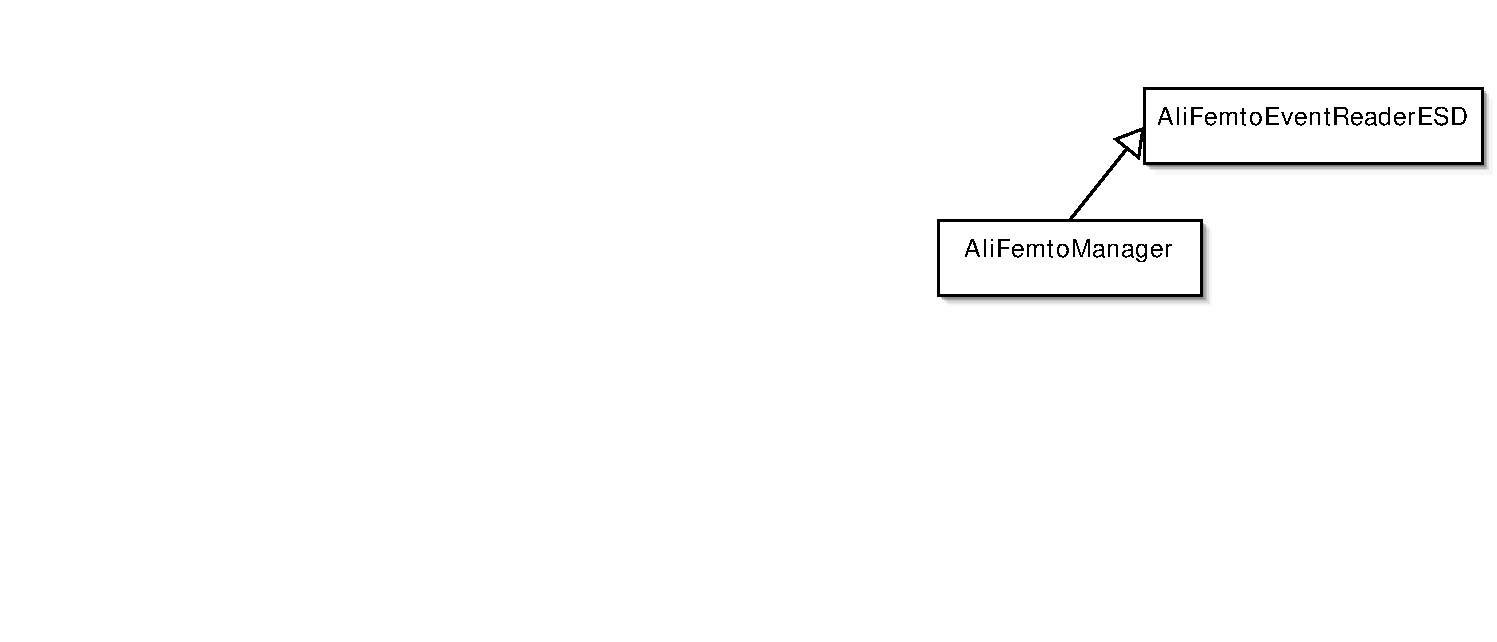
\includegraphics[width=\textwidth]{ExampleMacro1.pdf}
\caption{The preliminaries in a \AliFemto macro: loading of the libraries, instantiation of top-level structure, and
instantiating and plugging in a Reader.
The cartoon is meant so suggest the action of the macro commands; it is not a UML diagram.
\label{fig:exampleMacroGload}
}
\end{figure}

\begin{figure}[t]

\includegraphics[width=\textwidth]{ExampleMacro2.pdf}
\caption{The construction of a specific \name{AliFemtoAnalysis}, including its cuts and collection of three CorrFctn
objects.  The dark shaded region in the cartoon denotes a collection.
\label{fig:exampleFirstAnalysisStart}
}
\end{figure}

\begin{figure}[t]
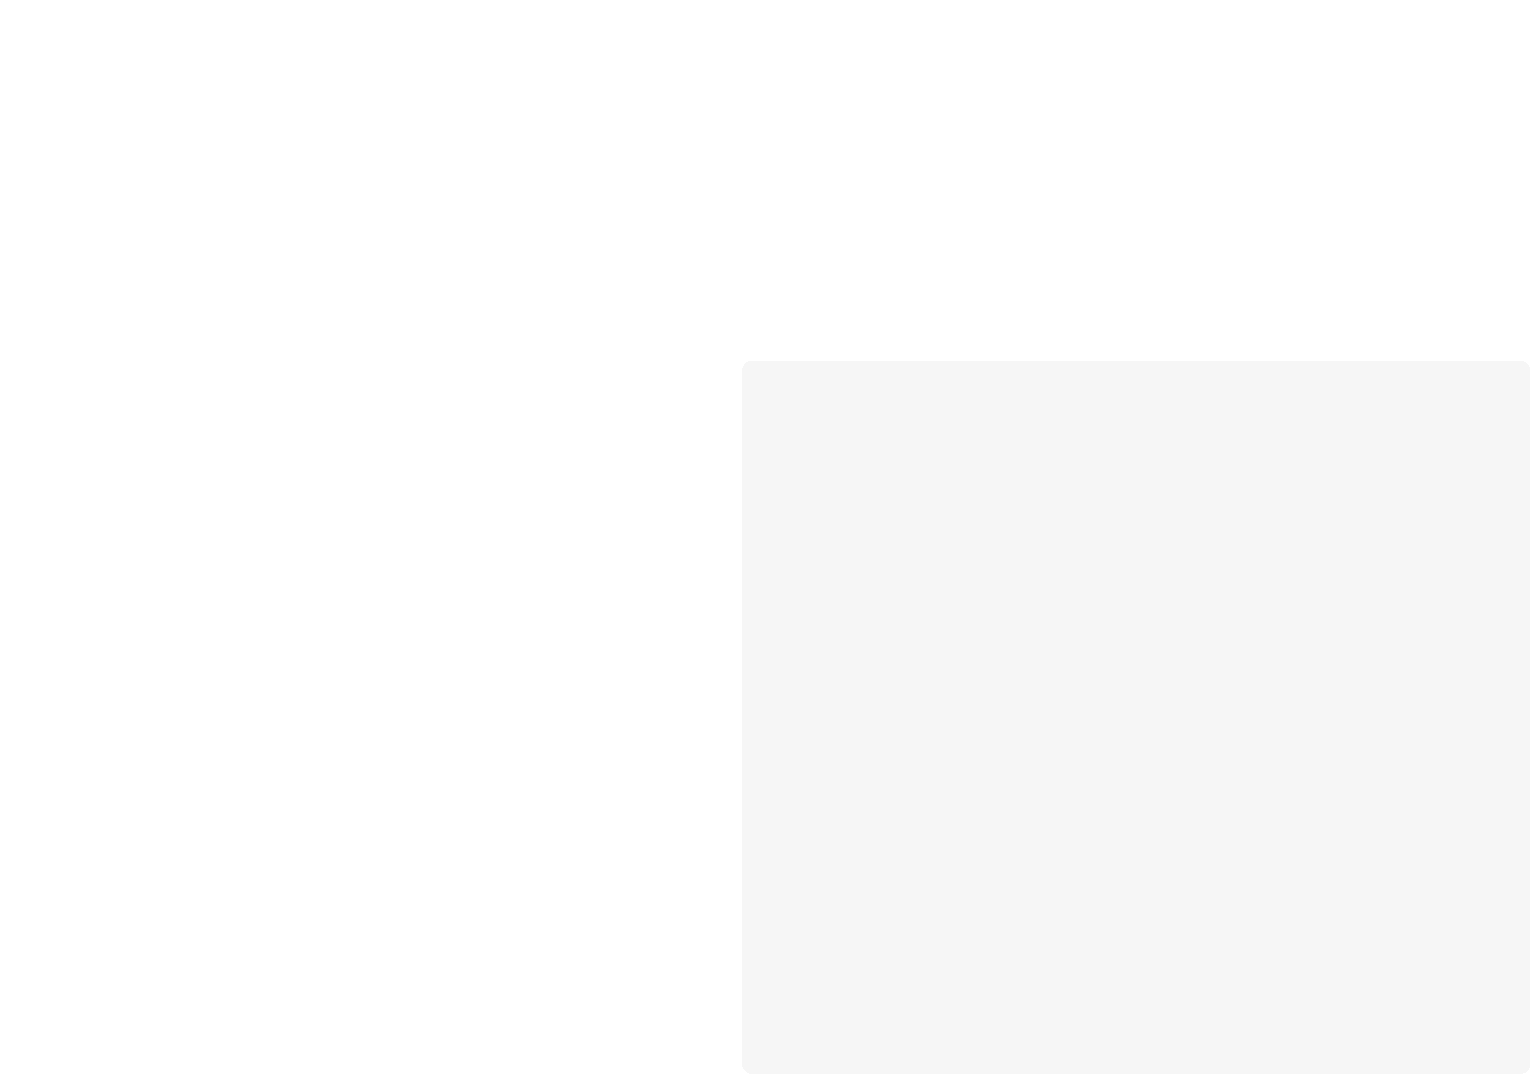
\includegraphics[width=\textwidth]{ExampleMacro3.pdf}
\caption{The final step in configuring the first Analysis is to set the number of events to mix when constructing
the ``background'' distribution.  This finished Analysis (dark grey box) is then added to the collection of Analyses
for the \name{AliFemtoManager} (large light grey box), thus making the connection between these objects.
\label{fig:exampleFirstAnalysisFinish}
}
\end{figure}

\begin{figure}[t]

\includegraphics[width=\textwidth]{ExampleMacro4.pdf}
\caption{A second Analysis is instantiated, configured, and added to the collection.  The same
proceedure is followed as for the fist Analysis (Figures~\ref{fig:exampleFirstAnalysisStart}
and~\ref{fig:exampleFirstAnalysisFinish}), though the two Analyses know nothing about each other.
\label{fig:exampleSecondAnalysis}
}
\end{figure}

\begin{figure}[t]

\includegraphics[width=\textwidth]{ExampleMacro5.pdf}
\caption{Construction of the AliFemto study complete, event looping is trivial.  Note that all
interaction with the code is through only a few methods of the AliFemtoManager object.
\label{fig:exampleEventLoop}
}
\end{figure}

Figure~\ref{fig:exampleMacroGload} shows the beginning of the macro.  
As usual in a root macro, libraries are loaded first.  For the femtoscopic analysis itself, only the AliFemto and AliFemtoUser
libraries need be loaded.  All internal \AliFemto classes such as \name{AliFemtoPair} are found in the AliFemto directory.
That directory also has a few simple CorrFcn, Reader, and Cut classes.  The user will probably want to start with these and
elaborate upon them; in this case, her new classes should go into the AliFemtoUser area.

In this example
we use the specific \name{AliFemtoEventReader}-derived class \name{AliFemtoEventReaderESD}; not surprisingly, this Reader needs
the ESD library loaded as well.



Since all Readers are user-written, their configuration
methods will be specific to the class used.  This is as it should be, since attempts to ``foresee'' all possible
uses of the Reader classes will ultimately result in limitations later on, and sloppy work-arounds.

The \name{AliFemtoManager} is instantiated; note that its pointer is declared outside the scope of the macro, at the top.
Finally, the \name{AliFemtoEventReaderESD} object is ``plugged in'' to the \name{AliFemtoManager}.  This is indicated by the arrow
in the cartoon; recall that this is not a UML diagram.

\subsubsection{Adding Analyses}
%--------------------- Example Step 2 ----------------------


In Figure~\ref{fig:exampleFirstAnalysisStart} we see construction of a specific Analysis  (c.f.
Section~\ref{sec:analysisLevel}).
An \name{AliFemtoAnalysis}-derived class, \name{AliFemtoVertexAnalysis}, is
instantiated.  (For reference, this class takes care to ``mix'' only those events close to each other in
primary vertex position; it is very commonly used.)  All configuration (vertex range, number of bins) takes
place in the constructor, in this specific class.

The Cuts are (i) instantiated, (ii) configured, and (iii) ``plugged into'' this Analysis.
Finally, three correlation functions are instantiated, configured, and added to the collection
of CorrFctns for this analysis.  (The collection is suggested by the dark-shaded box in the cartoon.)
We note that one of the CorrFctn classes there is \name{OpeningAngleCorrFctn}.  The fact that its name
does not begin with ``AliFemto'' is a clue that this class is user-written, for her own purposes; it would
not be included in ALICE nightly builds and would sit in the AliFemtoUser area.

Two notes:  Firstly, we see that the same AliFemtoTrackCut is used for both the first and second particle-- this
is an analysis of identical pions.  Secondly, as mentioned in  Section~\ref{sec:AliFemtoParticleCuts}, all AliFemtoParticleCuts
{\it must} define a particle mass.  This is not special to this specific example.

%--------------------- Example Step 3 ----------------------


In Figure~\ref{fig:exampleFirstAnalysisStart}, the conglomeration of Analysis-related objects is not related to
the AliFemtoManager instantiated in the previous Figure.  In Figure~\ref{fig:exampleFirstAnalysisFinish}, the connection
is made.  Firstly, the ``final detail'' for the Analysis is completed-- the number of events to mix for the reference
distribution is set, and the now-fully-configured Analysis is added to the collection of Analyses (denoted by the large
grey box).

%--------------------- Example Step 4 ----------------------


The structure is now complete in principle-- a useful correlation study may proceed.
We may add one or more completely seperate Analyses, if we wish.  This is shown in
Figure~\ref{fig:exampleSecondAnalysis}.  The only points here are that the second
(and any subsequent) Analyses are set up similarly to the first one discussed above, and
there is no connection the Analyses in the AliFemtoManager's collection of Analyses.


\subsubsection{Processing data}
\label{sec:ProcessingData}
%--------------------- Example Step 5 ----------------------


Finally, Figure~\ref{fig:exampleEventLoop} moves beyond construction of the collection
of objects, and commands a processing of the data.  We note that all ``external'' interaction
is with the AliFemtoManager class.  If the Reader needs to interact with the ``outside world''
(e.g. by opening a file or pointing to a location in memory), then it is up to that specific
class, using its own specific methods, to take care of that.

In Figure~\ref{fig:exampleEventLoop}, the processing is ordered within a ``pure root'' macro
directly.  This can be different in other frameworks.  For example, in the STAR Maker schema~\cite{StarMaker},
the AliFemtoManager Init(), ProcessEvent(), Report() and Finish() methods will be invoked by the AliFemtoMaker
Init(), Make(), and Finish() methods.  Indeed, the AliFemtoMaker does almost nothing else than perform these
simple invocations.


\section{Code Organization}


\subsection{Directory structure: core and user classes}
\label{sec:coreUser}

The femtoscopy analysis effort in ALICE falls in the soft physics working group (PWG2).
Thus, when checking out the full \AliRoot from \cvs, it will be found in the {\tt PWG2/FEMTOSCOPY/}
area.  (One may also check out only PWG2 files using\\
{\tt cvs -qz2 -d :pserver:cvs@alisoft.cern.ch:/soft/cvsroot co PWG2}.\\  This is useful if running
\AliFemto in ``standalone'' mode.)

In this directory are found two subdirectories.  The first is {\tt AliFemto/},
which holds about 80 classes (as of \today), such as \name{AliFemtoManager}, \name{AliFemtoPair}, etc.
It also holds all of the base classes for user-derived code (e.g. \name{AliFemtoCorrFctn}) and one
or two simple examples of classes which derive from these (e.g. \name{AliFemtoQinvCorrFctn}).  These
last might be useful templates for users writing more sophisticated Cuts, CorrFctns, Readers, Analyses, etc.
The {\tt AliFemto/} subdirectory is included in the official nightly build.  Files there must obey
ALICE coding standards, and limited \cvs access is anticipated.

The second directory is {\tt AliFemtoUser/}.  Files in this subdirectory are not included in the nightly
build.  This area is meant to be a repository for user code, typically Cuts, CorrFctns, etc, which might
be of interest to others working on some analysis.  It is \cvs archived, and widespread read/write \cvs access
is anticipated.

Seperate shared object (.so) libraries are built for the {\tt AliFemto/} and {\tt AliFemtoUser/}
area; c.f. the macro snip in Figure~\ref{fig:exampleMacroGload}.


\section{Known problems}

As of \today, there are no known problems with \AliFemto.  However, this Users' Guide is incomplete, in that
it does not discuss so-called ``theoretical'' correlation studies covered in the \name{AliFemtoModel*} classes.
This will be remedied in the next version of the Users' Guide.  In the meantime, see an excellent tutorial
on the subject on the ALICE femtoscopy webpage\\
 {\tt http://aliceinfo.cern.ch/Collaboration/PhysicsWorkingGroups/PWG2/Femtoscopy/}.



\clearpage

\part{Reference Manual}
\label{part:RefMan}

The Reference Manual is being finalized.

\clearpage



%%%%%%%%\section{References}
\begin{thebibliography}{99}

 \bibitem{UMLreference}
   The Unified Modeling Language (UML), 
   http://www.omg.org/technology/documents/formal/uml.htm ;
   http://en.wikipedia.org/wiki/Unified\_Modeling\_Language

\bibitem{Lisa:2005dd}
  M.~A.~Lisa, S.~Pratt, R.~Soltz and U.~Wiedemann,
  %``Femtoscopy in relativistic heavy ion collisions,''
  Ann.\ Rev.\ Nucl.\ Part.\ Sci.\  {\bf 55}, 357 (2005)
  [arXiv:nucl-ex/0505014].
  %%CITATION = NUCL-EX 0505014;%%

\bibitem{HanburyBrown:1954}
  Hanbury-Brown, R., and Twiss, R.Q.
  %''A new type of interferometer for use in radio-astronomy'',
  Phil. Mag. {\bf 45}, 663 (1954).

\bibitem{Goldhaber:1960sf}
  Goldhaber, Gerson and Goldhaber, Sulamith and Lee, Won-Yong
                  and Pais, Abraham, 
  %''Influence of Bose-Einstein statistics on the antiproton
                  proton  annihilation process''
  Phys. Rev. {\bf 120} 300 (1960).

\bibitem{Lednicky:2002fq}
   Lednicky, R.,
   %''Progress in correlation femtoscopy,''
   nucl-th/0212089


\bibitem{StarMaker}
%Unfortunately, the best (!?!?) documentation of the basic STAR Maker analysis framework is
%a brief presentation by Victor Perevoztchikov which may be found on the STAR computing
%tutorial website:
Tutorial by Victor Perevoztchikov 
http://www.star.bnl.gov/STAR/comp/train/tut/Maker-in-STAR/Victor-Makers.html

\end{thebibliography}


%%%%%%%%%%%%%%%%%%%%%%%%%%%%%%%%%%%%%%%%%%%%%%%%%%%%%%%%%%%%%%%%%%%%
%
% The End
%
%%%%%%%%%%%%%%%%%%%%%%%%%%%%%%%%%%%%%%%%%%%%%%%%%%%%%%%%%%%%%%%%%%%%

\printindex

\end{document}
